% Autor: Leonhard Segger, Alexander Neuwirth
% Datum: 2017-10-30
\documentclass[
	% Papierformat
	a4paper,
	% Schriftgröße (beliebige Größen mit „fontsize=Xpt“)
	12pt,
	% Schreibt die Papiergröße korrekt ins Ausgabedokument
	pagesize,
	% Sprache für z.B. Babel
	ngerman
]{scrartcl}

% Achtung: Die Reihenfolge der Pakete kann (leider) wichtig sein!
% Insbesondere sollten (so wie hier) babel, fontenc und inputenc (in dieser
% Reihenfolge) als Erstes und hyperref und cleveref (Reihenfolge auch hier
% beachten) als Letztes geladen werden!

% Silbentrennung etc.; Sprache wird durch Option bei \documentclass festgelegt
\usepackage{babel}
% Verwendung der Zeichentabelle T1 (Sonderzeichen etc.)
\usepackage[T1]{fontenc}
% Legt die Zeichenkodierung der Eingabedatei fest, z.B. UTF-8
\usepackage[utf8]{inputenc}
% Schriftart
\usepackage{lmodern}
% Zusätzliche Sonderzeichen
\usepackage{textcomp}

% Mathepaket (intlimits: Grenzen über/unter Integralzeichen)
\usepackage[intlimits]{amsmath}
% Ermöglicht die Nutzung von \SI{Zahl}{Einheit} u.a.
\usepackage{siunitx}
% Zum flexiblen Einbinden von Grafiken (\includegraphics)
\usepackage{graphicx}
% Abbildungen im Fließtext
\usepackage{wrapfig}
% Abbildungen nebeneinander (subfigure, subtable)
\usepackage{subcaption}
% Funktionen für Anführungszeichen
\usepackage{csquotes}
% Zitieren, Bibliographie
\usepackage{biblatex}

\usepackage{subcaption}


% Zur Darstellung von Webadressen
\usepackage{url}
%chemische Formeln
\usepackage[version=4]{mhchem}
% siunitx: Deutsche Ausgabe, Messfehler getrennt mit ± ausgeben
\usepackage{floatrow}
\floatsetup[table]{capposition=top}
\usepackage{float}
% Verlinkt Textstellen im PDF-Dokument
\usepackage[unicode]{hyperref}
% "Schlaue" Referenzen (nach hyperref laden!)
\usepackage{cleveref}
\sisetup{
	locale=DE,
	separate-uncertainty
}
\bibliography{14Mo_O7_23-04-2018_References}

\begin{document}
	
	\begin{titlepage}
		\centering
		{\scshape\LARGE Versuchsbericht zu \par}
		\vspace{1cm}
		{\scshape\huge O7 - Beugung am Spalt, Doppelspalt und Gitter \par} %TODO Anpasen
		\vspace{2.5cm}
		{\LARGE Gruppe 14Mo \par}
		\vspace{0.5cm}
		
		{\large Alexander Neuwirth (E-Mail: a\_neuw01@wwu.de) \par}
		{\large Leonhard Segger (E-Mail: l\_segg03@uni-muenster.de) \par}
		\vfill
		
		durchgeführt am 23.04.2018\par %TODO Anpassen
		betreut von\par
		{\large Lukas Britt} %TODO Anpassen
		
		\vfill
		
		{\large \today\par}
	\end{titlepage}
	\tableofcontents
	\newpage

	\section{Kurzfassung}
	%TODO Hypothese	und deren Ergebnis
	%TODO Ergebnisse, auch Zahlen, mindestens wenn's halbwegs Sinn ergibt
	%TODO Was wurde gemacht
	
	%TODO Einleitungssatz
	Für die Wellenlänge des Laserlichts erwarten wir eine Wellenlänge von \SI{630}{\nano \meter} bis \SI{680}{\nano \meter}, da dies die Angabe auf dem Laser war.
	Bei der Intensitätsverteilung eines Einzelspalts ist ein Verlauf gemäß der Funktion $ \left( \sin \beta / \beta \right) ^2 $ zu erwarten. %TODO evtl. vgl. Bild von Funktion
	Beim Doppelspalt erwartet man eine Oszillation mit der Intensitätsverteilung des Einzelspalts mit selber Spaltbreite als einhüllende Funktion.
	Der Vergleich der Intensitätsverteilung von Doppelspalten mit verschiedenen Spaltabständen und Spaltbreiten sollte sich in der Erwartung wie in der Theorie verhalten (vgl. \cref{Doppelspaltvergleich}). %TODO in Diskus aufführen Abhängigkeit g,b
	Außerdem erwarten wir bei Mehrfachspalten einen Anstieg der Intensität der Hauptmaxima mit der Anzahl der Spalte.
	Dies konnte für kleine Spaltzahlen bestätigt werden.
	Die Halbwertsbreite der Hauptmaxima hat wie erwartet mit steigender Spaltzahl zugenommen.
	
	\section{Methoden}
	In \cref{optischeBank} ist er Aufbau des Experiments illustriert.
	An einem Ende der optischen Bank befindet sich ein Diodenlaser und davor ein Polarisator und der Halter für Spalte.
	Am anderen Ende der optischen Bank ist eine durch eine Kurbel senkrecht zu optischen Bank zu bewegende Photodiode angebracht.
	Die Halterung der Photodiode ist über ein Seil mit einem Rad verbunden, um die Intensitätsmessung der Diode mit der Position der Diode im Strahlengang zu verbinden.
	Nun kann eine Spaltanordnung in die Halterung gebracht werden und durch Bewegung der Photodiode über die optische Bank die Intensitätsverteilung der Spalte bestimmt werden.
	Dies wurde für unterschiedliche Spalte durchgeführt. %TODO Neukalibrierung erwähnen?
	
	\begin{figure}[H]
		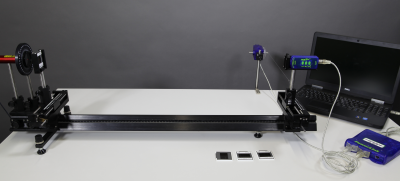
\includegraphics[width=0.7\textwidth]{optischeBank}
		\centering
		\caption{Aufbau der optischen Bank. Auf der linken Seite sind Laser und Beugungsanordnung und auf der rechten Seite die Photodiode zu sehen.\cite{optischeBank} }
		\label{optischeBank}
		\centering
	\end{figure} 
	
	\section{Ergebnisse und Diskussion}
	%TODO Datenanalyse -> Überschrift?
	%TODO Unsicherheiten
	

	\subsection{Beobachtung}
	
	\subsubsection{Bestimmen der Wellenlänge des Laserlichts}
	In \crefrange{Einzelspalt0-075mm}{Einzelspalt0-400mm} sind für Einzelspalte der Breite $b$ = \SI{0,075}{mm}, \SI{0,15}{mm} und \SI{0,4}{mm} die Intensitätsverteilungen dargestellt. 
	Die Unsicherheit der Breite wird mit 1\% abgeschätzt.
	Mit \cref{einzelminmax} lässt sich aus der Positionen von einem Minimum ( $m$ = $\pm1$, $\pm 2$, ...) oder Maximum ( $m$ = $\pm1,5$, $\pm 2,5$, ...) die Wellenlänge $\lambda$ berechnen. 
	
	\begin{equation}
		\sin(\vartheta) = m \frac{\lambda}{b}
		\label{einzelminmax}
	\end{equation}
	Der Winkel $\sin(\vartheta)$ ergibt sich nach \cref{dreieck} aus dem Abstand des Gitters zum Schirm $d$ = \SI{0,78 +- 0,009}{m} und der Position des Extremas $x$. 
	\begin{equation}
		\sin(\vartheta) = \frac{x}{\sqrt{d^2 + x^2}}
		\label{dreieck}
	\end{equation}
	Für die Wellenlänge folgt:
	\begin{equation}
		\lambda = \frac{b}{m\sqrt{(d/x)^2 + 1}}
	\end{equation}
	\begin{equation}
	u(\lambda) = \frac{\lambda}{d^2+x^2} \sqrt{\left( \frac{d^2}{x} u(x)\right)^2 + \left( \frac{(d^2+ x^2)}{b}u(b) \right) ^2 + \left( du(d) \right)^2}
	\end{equation}
	
	\begin{table}[H]
		\centering
		\begin{tabular}{ c | c | c | c }
			$b$ & $m$ &  $|x|$ & $\lambda$ \\ \hline
			\SI{0,075 +- 0,0008}{mm} & -1,5 & \SI{10 +- 0,2}{mm} & \SI{641 +- 16}{nm} \\
			\SI{0,075+- 0,0008}{mm} & -1,0 & \SI{7,5 +- 0,2}{mm} & \SI{673+-22}{nm} \\
			
			\SI{0,150+- 0,0015}{mm} & 1,5 & \SI{5 +- 0,2}{mm} & \SI{641+-27}{nm} \\
			\SI{0,150+- 0,0015}{mm} & 1,0 & \SI{4 +- 0,2}{mm} & \SI{770+-40}{nm} \\
			\SI{0,150+- 0,0015}{mm} & -1,5 & \SI{4,9 +- 0,2}{mm} & \SI{628+-27}{nm} \\
			\SI{0,150+- 0,0015}{mm} & -1,0 & \SI{3,5 +- 0,2}{mm} & \SI{673+-40}{nm} \\
			
			\SI{0,150+- 0,0015}{mm} & 2,5 & \SI{9 +- 0,2}{mm} & \SI{692+-19}{nm} \\
			\SI{0,150+- 0,0015}{mm} & 2,0 & \SI{7 +- 0,2}{mm} & \SI{673+-22}{nm} \\
			\SI{0,150+- 0,0015}{mm} & -2,5 & \SI{8 +- 0,2}{mm} & \SI{615+-18}{nm} \\
			\SI{0,150+- 0,0015}{mm} & -2,0 & \SI{7 +- 0,2}{mm} & \SI{673+-22}{nm} \\
			
			\SI{0,400+- 0,004}{mm} & 1,5 & \SI{1,8 +- 0,02}{mm} & \SI{615+-16}{nm} \\
			\SI{0,400+- 0,004}{mm} & 1,0 & \SI{1,3 +- 0,02}{mm} & \SI{667+-14}{nm} \\
			\SI{0,400+- 0,004}{mm} & -1,5 & \SI{1,9 +- 0,02}{mm} & \SI{650+-12}{nm} \\
			\SI{0,400+- 0,004}{mm} & -1,0 & \SI{1,3 +- 0,02}{mm} & \SI{667+-14}{nm} \\
		\end{tabular}
		\caption{Aus Extrema ermittelte Wellenlängen für verschiedene Spaltbreiten.}
		\label{Einzelspalte} 
	\end{table}
	Der Mittelwert der Wellenlängen aus \cref{Einzelspalte} beträgt $\bar{\lambda}$ = \SI{663 +- 11}{nm}.
	%TODO zu klein?!? => nicht in eine Zeile => ?ANHANG?
	\begin{figure}[H]
		\centering
		\begin{subfigure}{.5\textwidth}
			\centering
			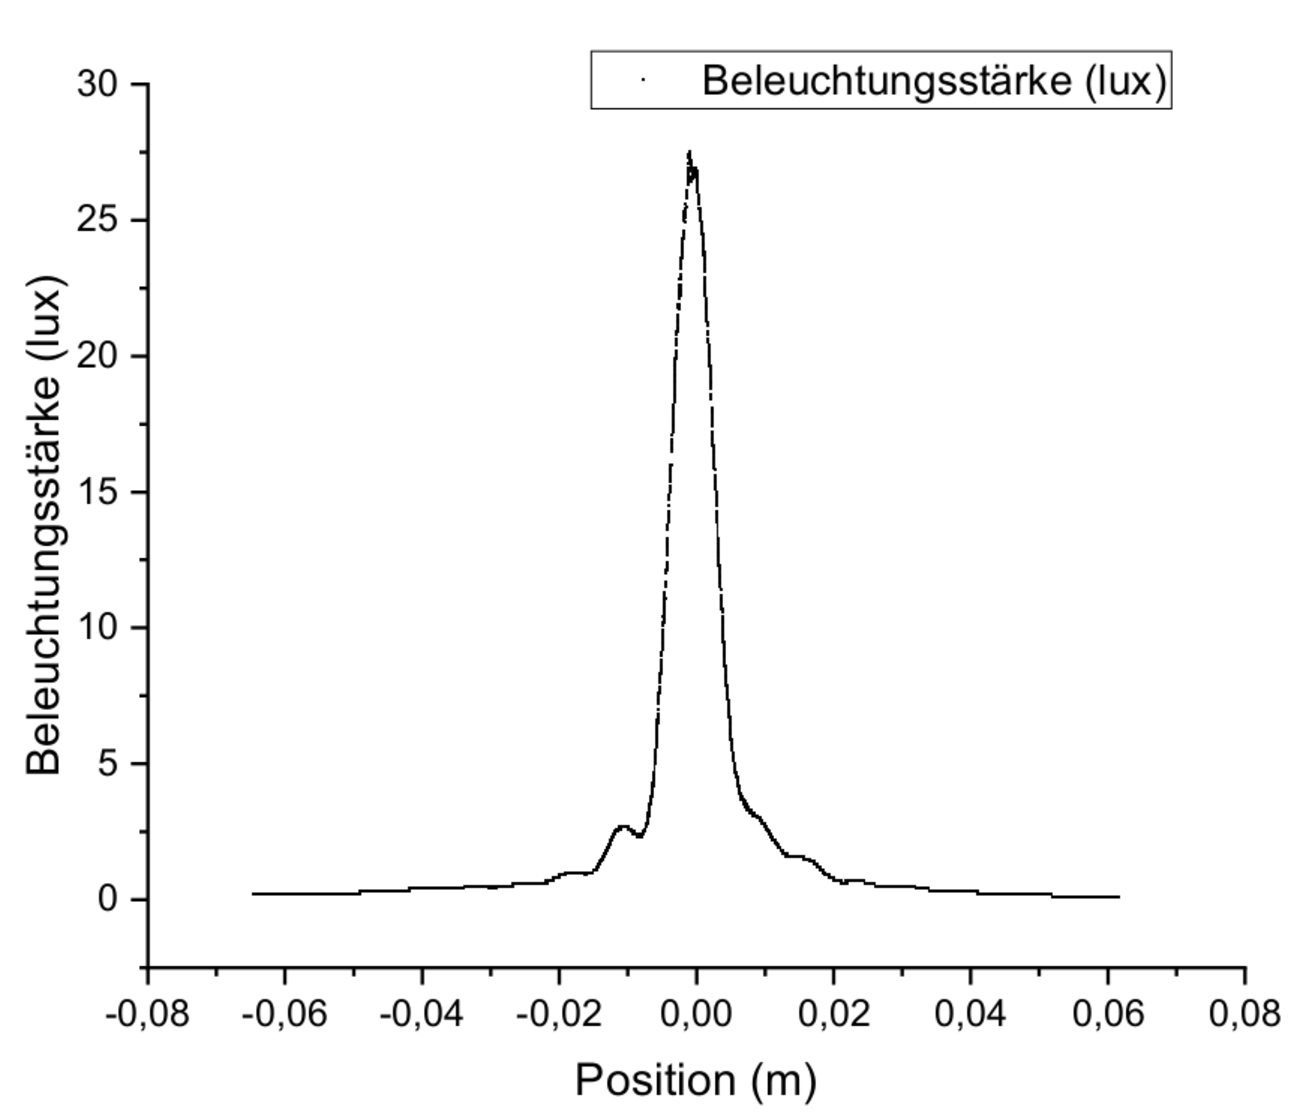
\includegraphics[width=1\linewidth]{Einzelspalt0-075mm}
			\caption{Gesamte Messung}	
		\end{subfigure}%
		\begin{subfigure}{.5\textwidth}
			\centering
			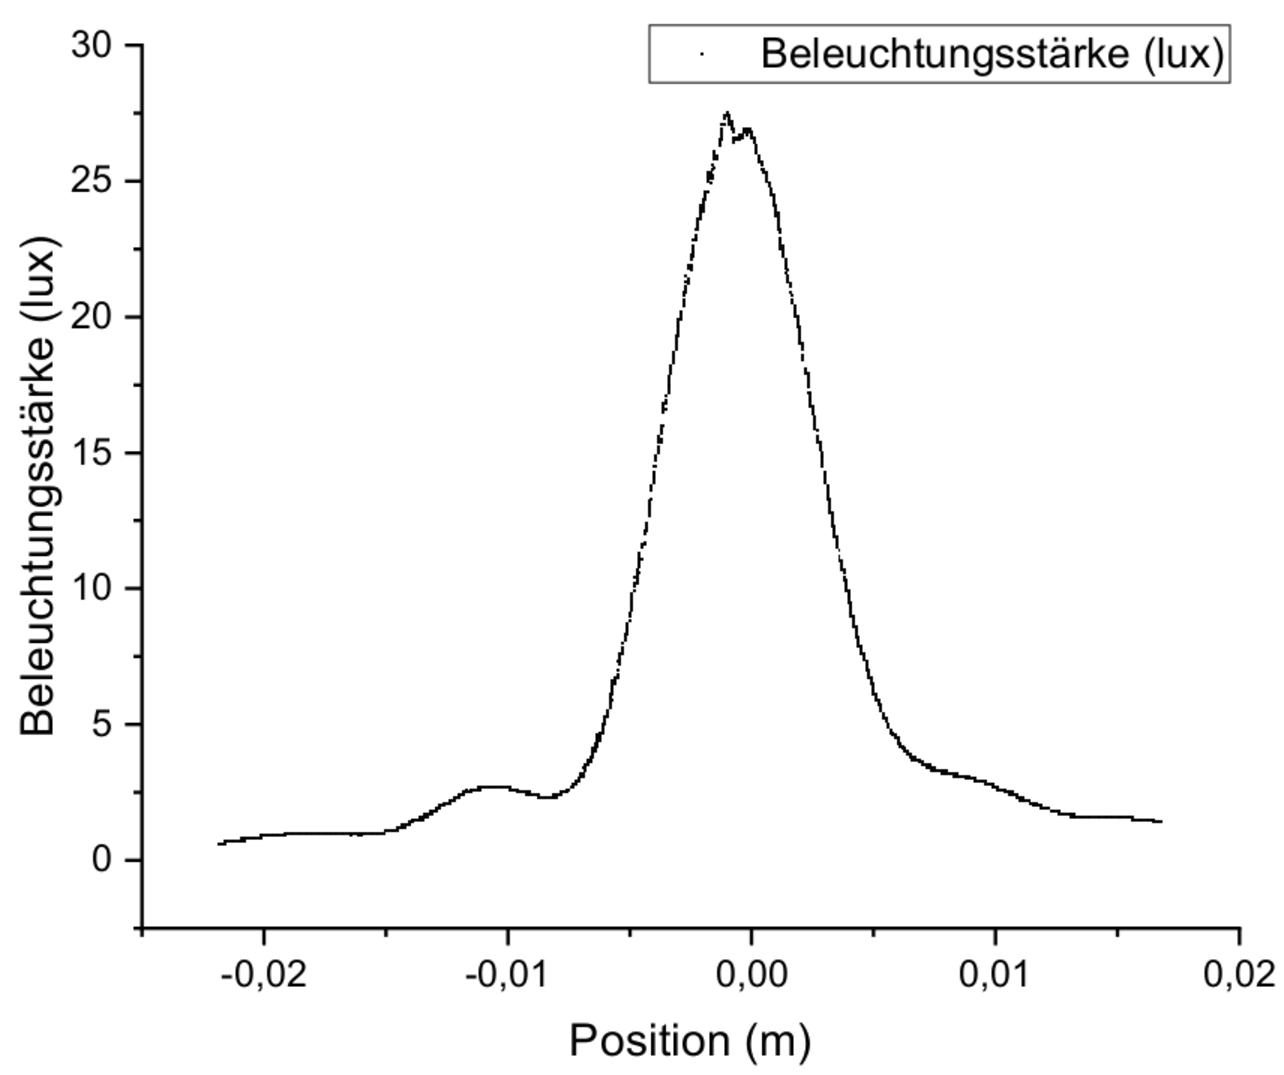
\includegraphics[width=1\linewidth]{Einzelspalt0-075mmZOOM}
			\caption{Extrema niedriger Ordnung}
		\end{subfigure}
		\label{Einzelspalt0-075mm}
		\caption{Intensitätsverteilung für einen Einzelspalt mit der Spaltbreite $b$ = \SI{0,075}{mm}.}
	\end{figure}	
	\begin{figure}[H]
		\centering
		\begin{subfigure}{.5\textwidth}
			\centering
			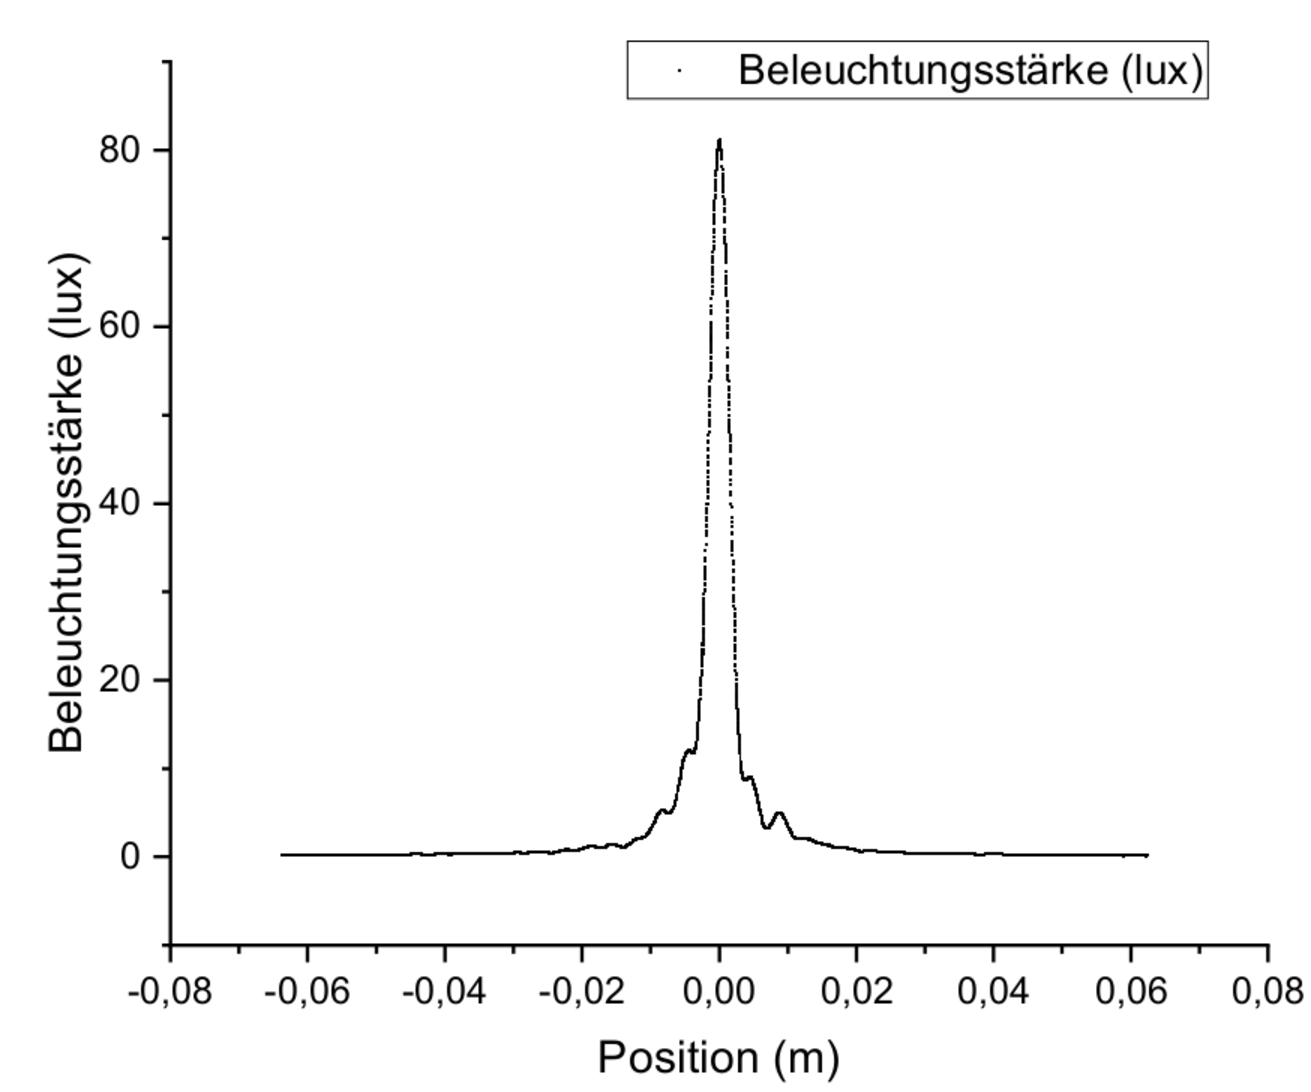
\includegraphics[width=1\linewidth]{Einzelspalt0-150mm}
			\caption{Gesamte Messung}	
		\end{subfigure}%
		\begin{subfigure}{.5\textwidth}
			\centering
			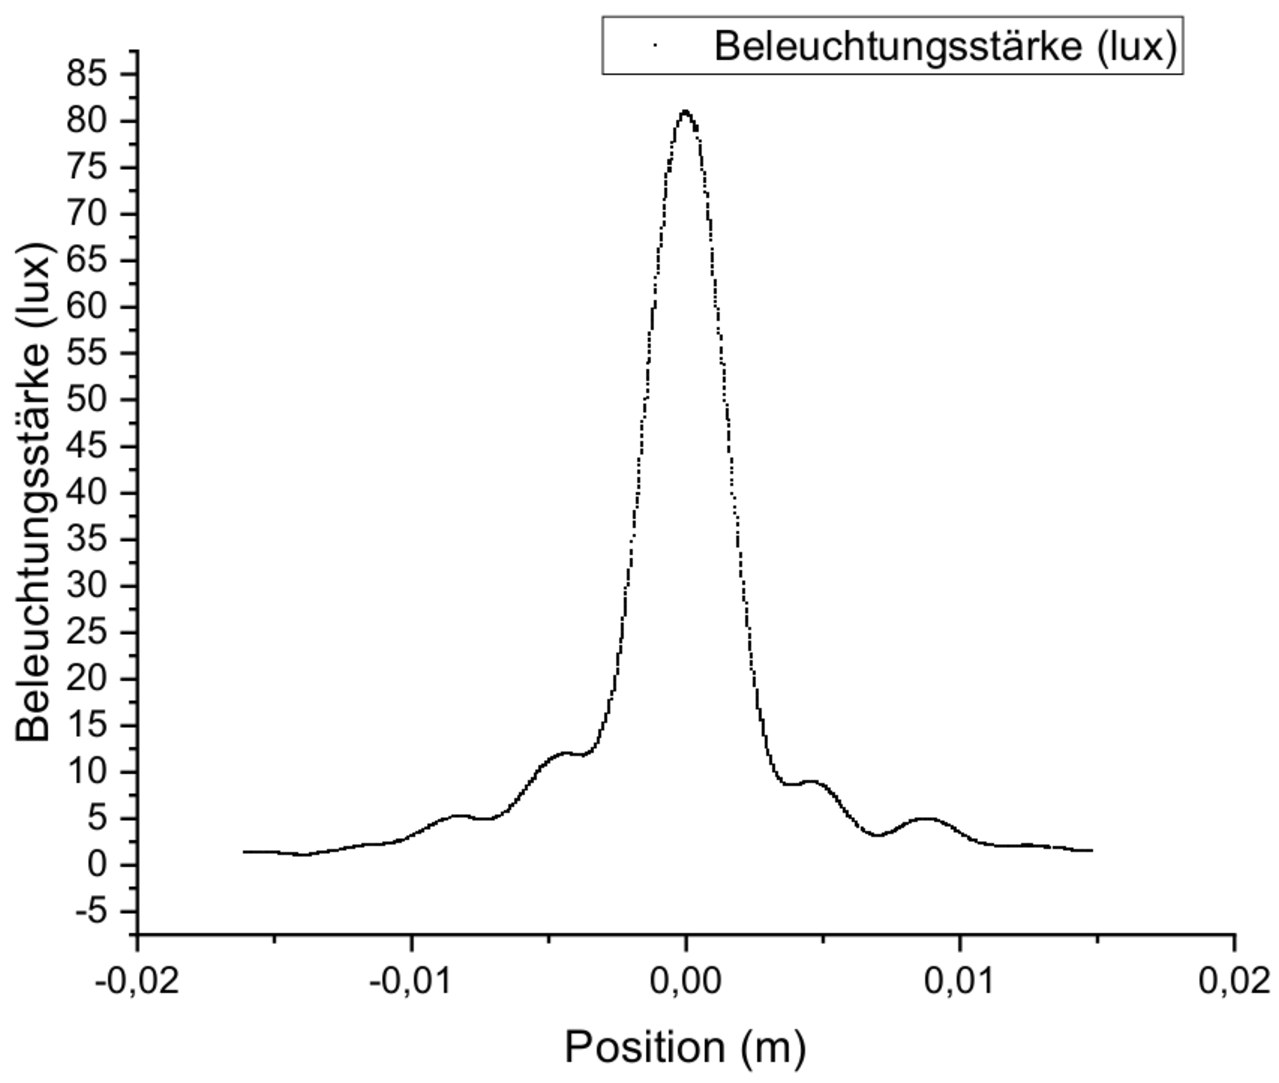
\includegraphics[width=1\linewidth]{Einzelspalt0-150mmZOOM}
			\caption{Extrema niedriger Ordnung}
		\end{subfigure}
		\label{Einzelspalt0-150mm}
		\caption{Intensitätsverteilung für einen Einzelspalt mit der Spaltbreite $b$ = \SI{0,15}{mm}.}
	\end{figure}	

	\begin{figure}[H]
		\centering
		\begin{subfigure}{.5\textwidth}
			\centering
			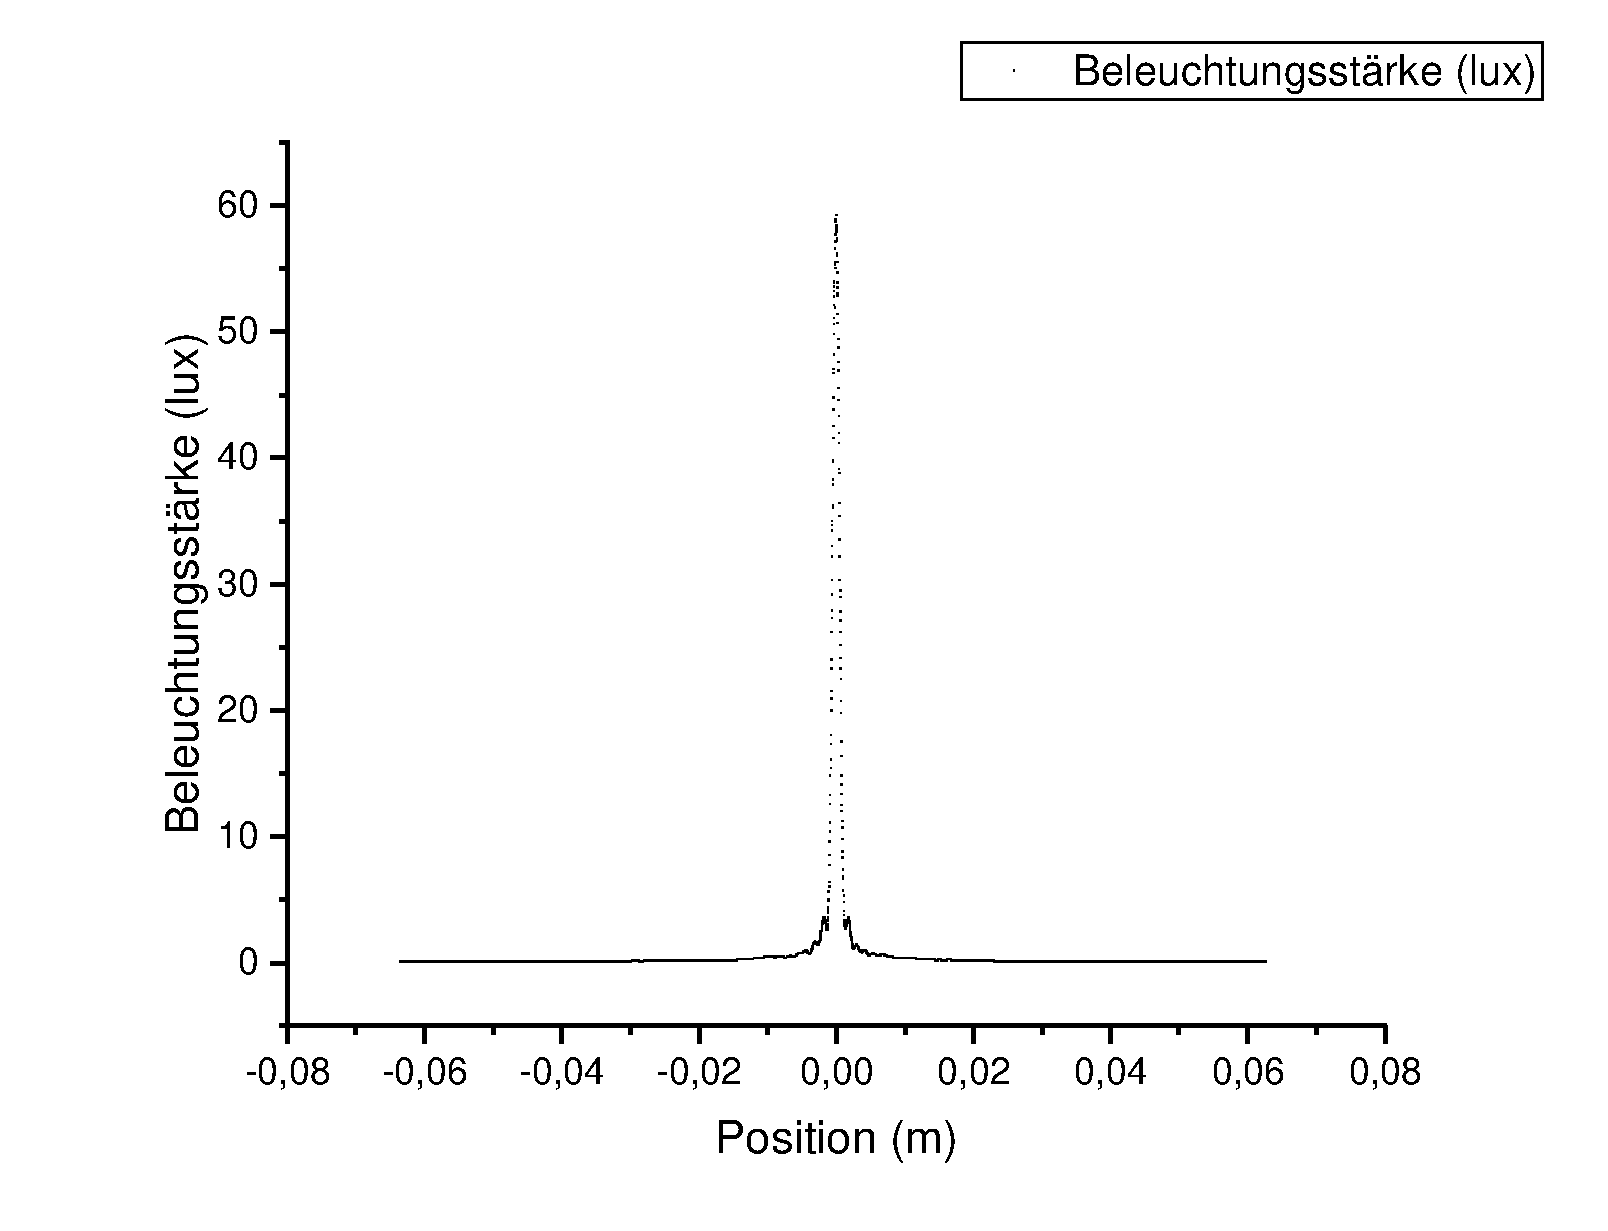
\includegraphics[width=1\linewidth]{Einzelspalt0-400mm}
			\caption{Gesamte Messung}	
		\end{subfigure}%
		\begin{subfigure}{.5\textwidth}
			\centering
			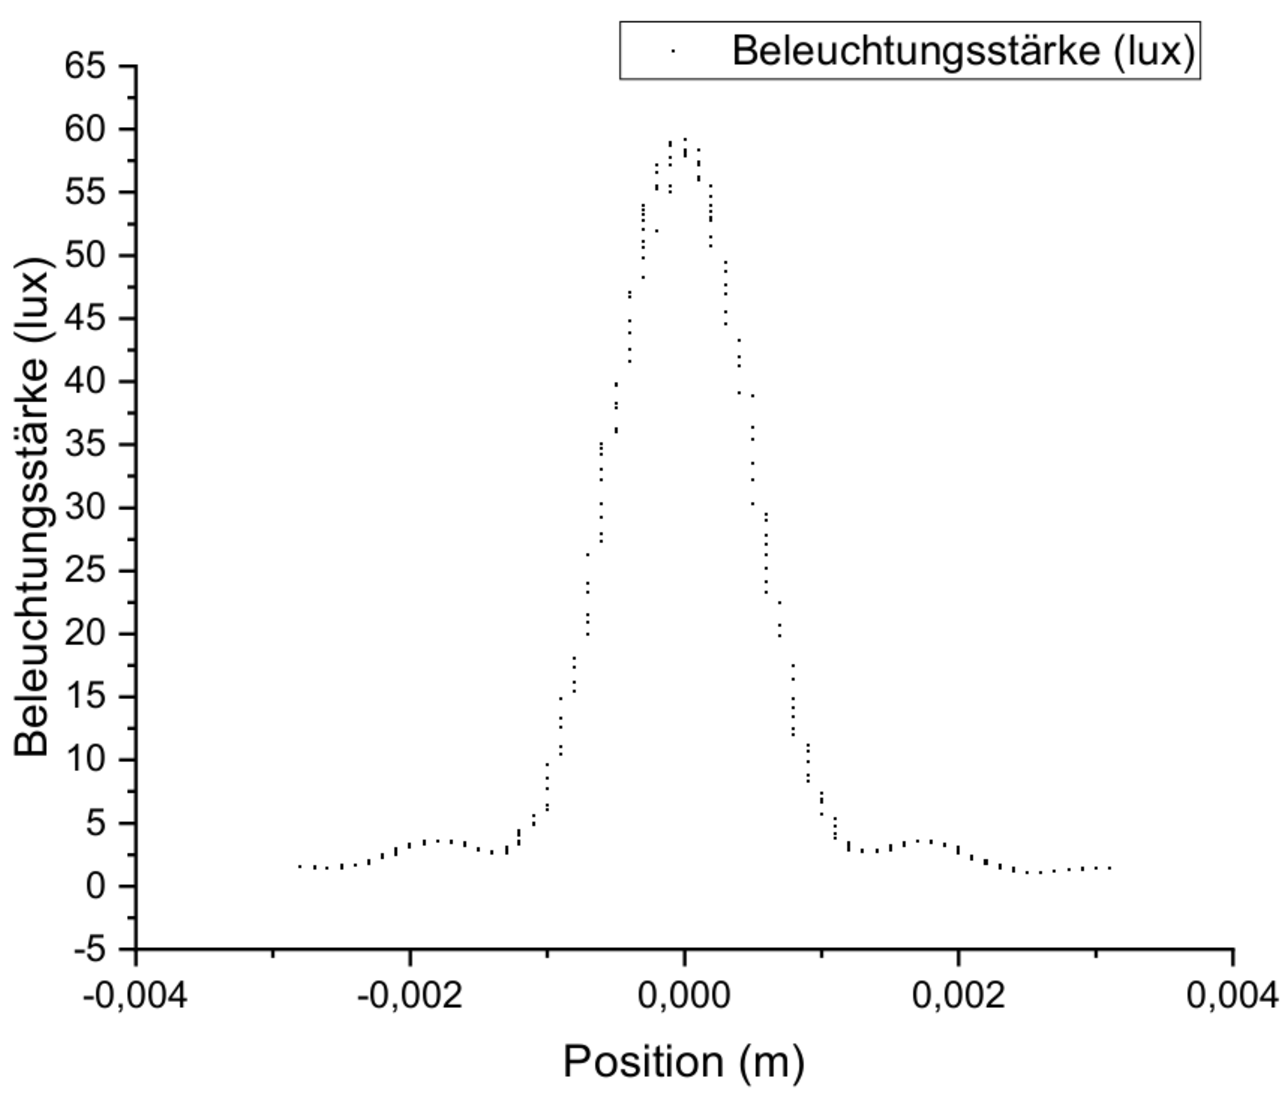
\includegraphics[width=1\linewidth]{Einzelspalt0-400mmZOOM}
			\caption{Extrema niedriger Ordnung}
		\end{subfigure}
		\label{Einzelspalt0-400mm}
		\caption{Intensitätsverteilung für einen Einzelspalt mit der Spaltbreite $b$ = \SI{0,4}{mm}.}
	\end{figure}

	\subsubsection{Gitterzeug} %TODO TITEL
	In \cref{GitterGraphen} sind die Intensitätsverteilungen von Mehrfachspalten mit $N$ = 3,4,5 und 40 dargestellt. 
	Zusätzlich sind in \cref{GitterTabelle} die Intensitäten der ersten zwei Hauptmaxima und deren Halbwertsbreite aufgeführt. 

	\begin{figure}[H]
		\centering
		\begin{subfigure}{.5\textwidth}
			\centering
			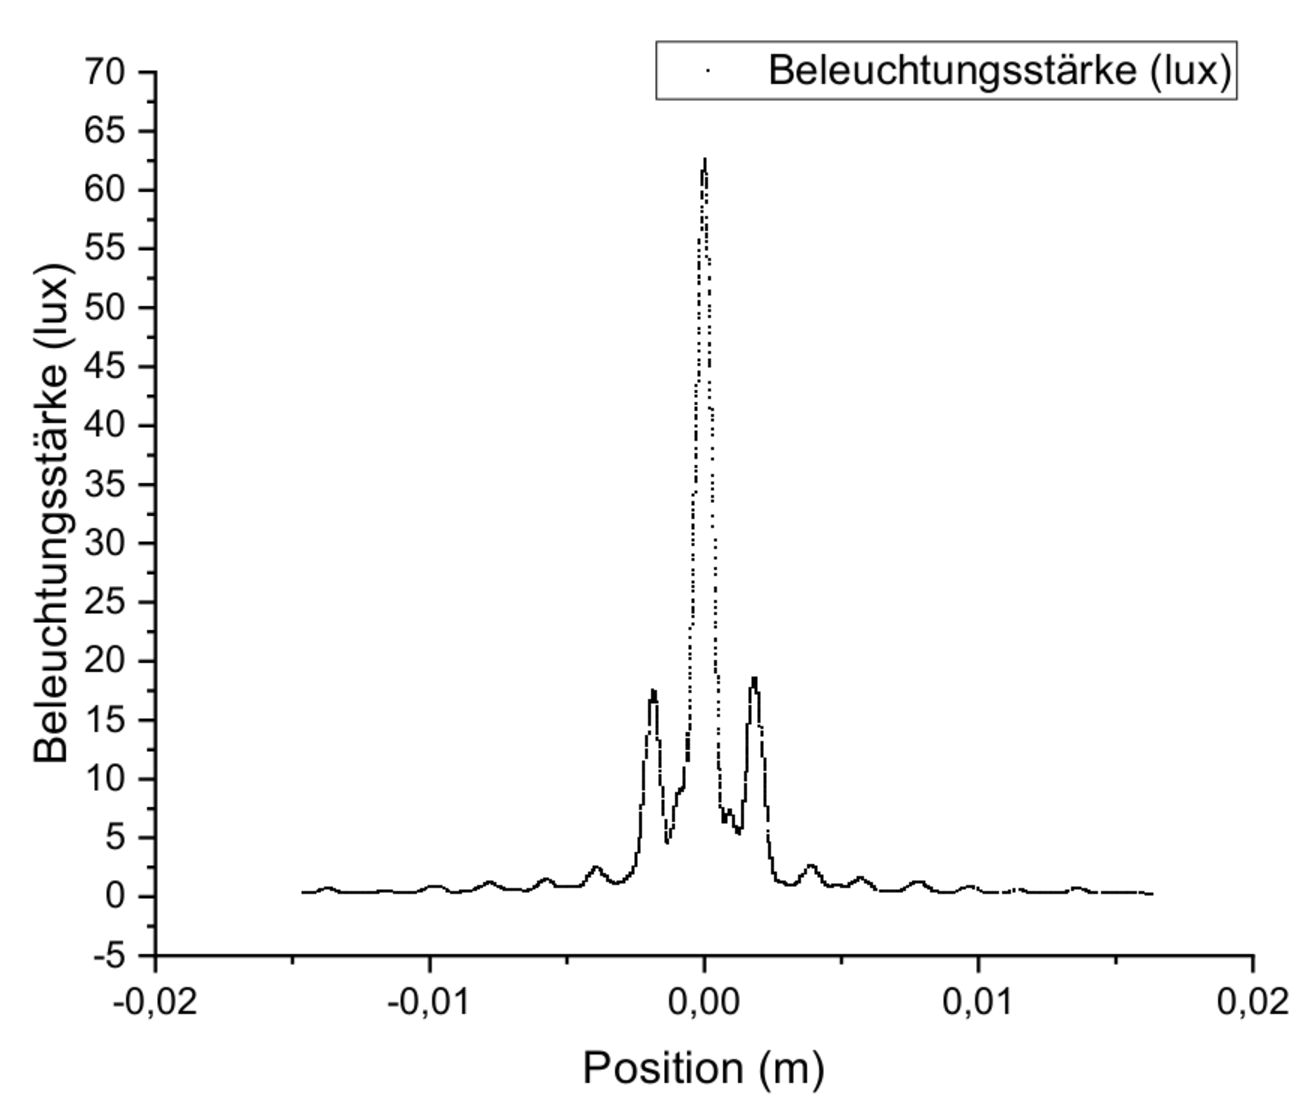
\includegraphics[width=1\linewidth]{GitterN3ZOOM}
			\caption{$N$=3}	
		\end{subfigure}%
		\begin{subfigure}{.5\textwidth}
			\centering
			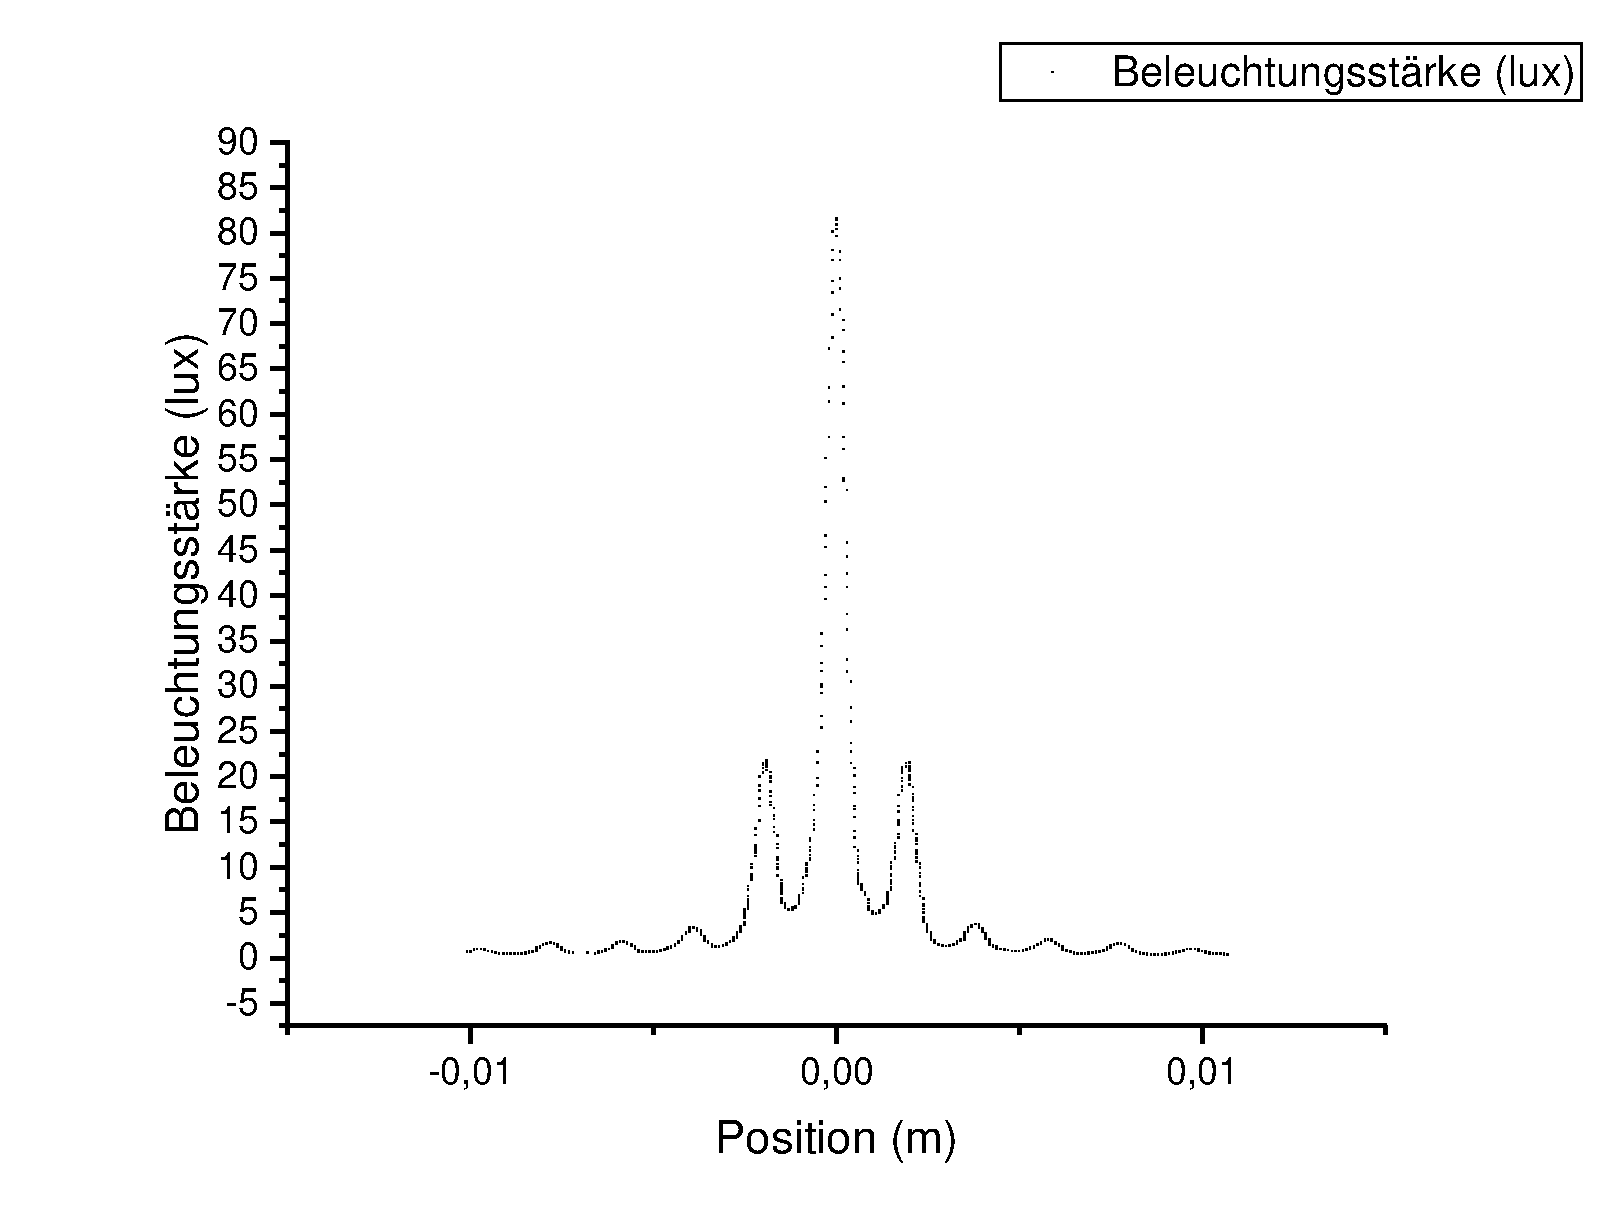
\includegraphics[width=1\linewidth]{GitterN4ZOOM}
			\caption{$N$=4}
		\end{subfigure}
		\begin{subfigure}{.5\textwidth}
			\centering
			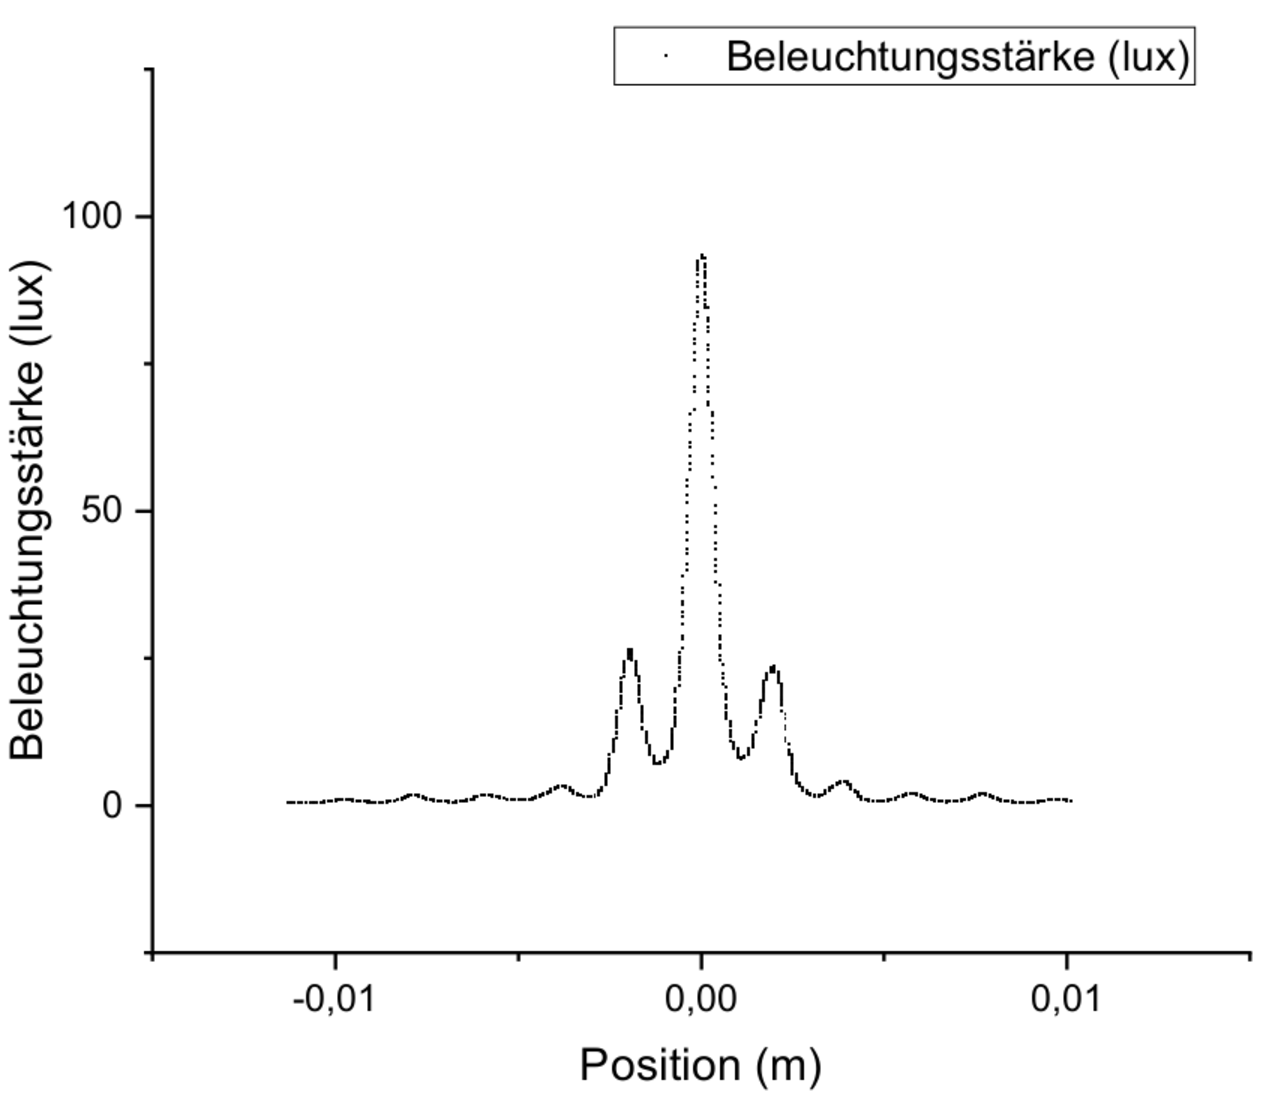
\includegraphics[width=1\linewidth]{GitterN5ZOOM}
			\caption{$N$=5}	
		\end{subfigure}%
		\begin{subfigure}{.5\textwidth}
			\centering
			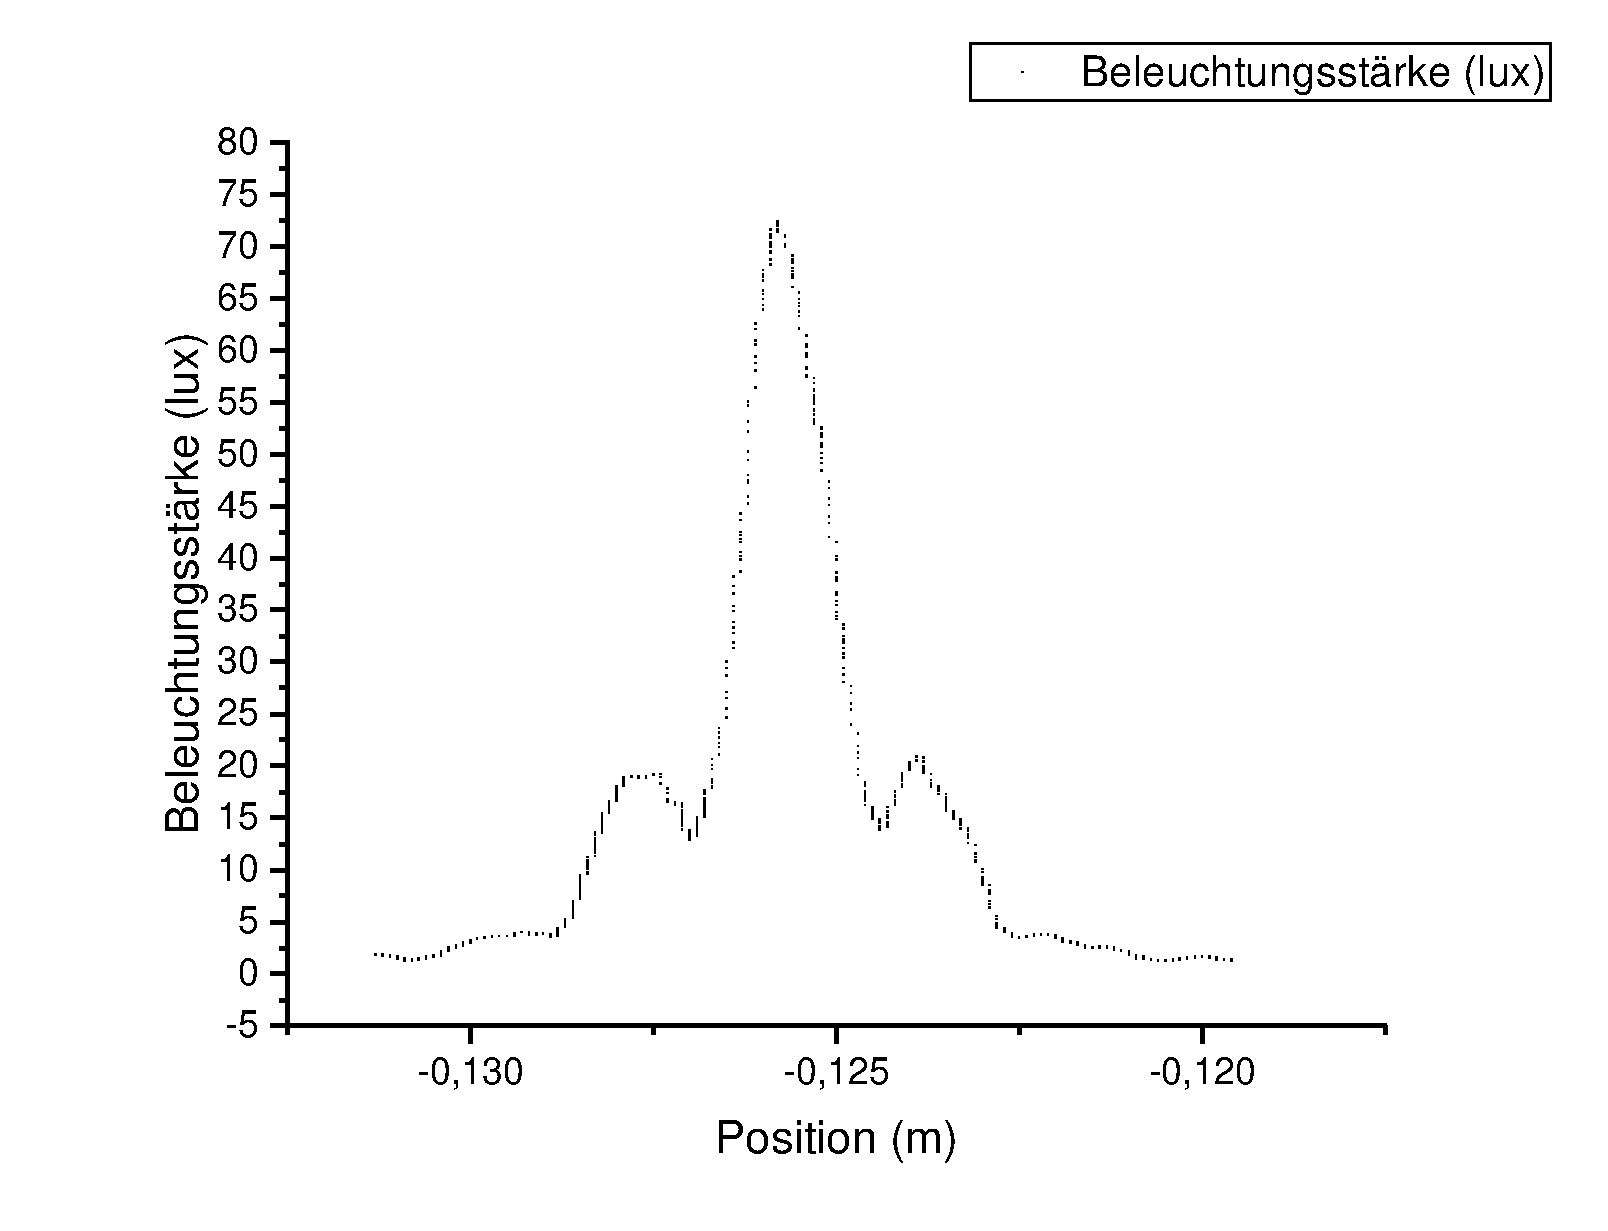
\includegraphics[width=1\linewidth]{GitterN40ZOOM}
			\caption{$N$=40}
		\end{subfigure}
		\caption{Intensitätsverteilungen verschiedener Mehrfachspalte  ($b$=\SI{0,15}{mm}, $g$=\SI{0,25}{mm}).}
		\label{GitterGraphen}
	\end{figure}

	

	\begin{table}[H]
		\centering
		\begin{tabular}{ c | c | c | c }
			$N$ &  Intensität 0.HM & Intensität 1.HM & Halbwertsbreite\\ \hline
			3 & \SI{62,6 +- 0,5}{lux} & \SI{18,5 +- 0,5}{lux} & \SI{0,0003+- 0,00001}{m} \\
			4 & \SI{81,6 +- 0,5}{lux} & \SI{21,8 +- 0,5}{lux} & \SI{0,0003+- 0,00001}{m} \\
			5 & \SI{93,4 +- 0,5}{lux} & \SI{23,7 +- 0,5}{lux} & \SI{0,0004+- 0,00001}{m} \\
			40& \SI{72,3 +- 0,5}{lux} & \SI{18,9 +- 0,5}{lux} & \SI{0,0007+- 0,00001}{m} \\
		\end{tabular}
		\caption{Intensitäten und Halbwertsbreiten der Maxima unterschiedlicher Mehrfachspalte ($b$=\SI{0,15}{mm}, $g$ = \SI{0,25}{mm}).}
		\label{GitterTabelle} 
	\end{table}
	
	Der Formfaktor wurde in dem Theorieteil wie folgt definiert: 
	\begin{equation}
		I_m \propto \left[\frac{\sin(m\pi b/g)}{m\pi b/g}\right]^2
	\end{equation}
	Folglich ist
	\begin{equation}
		I_1/I_0 = \left[\frac{\sin(\pi b/g)}{\pi b/g}\right]^2
	\end{equation}
	und es lässt sich das Verhältnis b/g bestimmen indem man $ \text{sinc}(\pi x)$ graphisch gleich dem Verhältnis $I_1/I_0$ setzt (unter der einschränkenden Voraussetzung $b/g<1$, da $\text{sinc}(x)$ sonst nicht umkehrbar ist).
	\begin{table}[H]
		\centering
		\begin{tabular}{ c | c | c | c | c }
			$N$ &  3 & 4 & 5 & 40\\ \hline
			$I_1/I_0$ & \SI{0,29+-0,008}{} & \SI{0,27+-0,006}{} & \SI{0,25+-0,005}{} & \SI{0,26+-0,007}{} \\
			$b/g$& \SI{0,57+-0,005}{} & \SI{0,59+-0,005}{} & \SI{0,60+-0,005}{} & \SI{0,60+-0,005}{} \\
		\end{tabular}
		\caption{Verhältnis zwischen erstem und nulltem Hauptmaximum. }
		\label{FormTabelle} 
	\end{table}
	\subsection{Diskussion}
	\subsubsection{Wellenlänge des Lasers}
	Aus den Extrema der Einzelspalte wurde eine Wellenlänge des Lasers von \SI{663\pm 11}{nm} bestimmt.
	Dies deckt sich mit der Angabe von \SI{630}{\nano \meter} bis \SI{680}{\nano \meter} auf dem Laser.
	
	\subsubsection{Vergleich von Einzelspalt und Doppelspalt}
	Wenn man die Intensitätsverteilung eines Einzelspalts mit $b=\SI{0,15}{mm}$ (vgl. \cref{Einzelspalt0-150mm}) mit einem Doppelspalt mit gleicher Spaltbreite vergleicht (vgl. \cref{Doppelspalt0-15mm}), lässt sich erkennen, dass die Maxima höherer Ordnung des Doppelspalts eine deutlich höhere Intensität verglichen mit dem Maxima nullter Ordnung haben als beim Einzelspalt.
	Außerdem liegen die Maxima bei unterschiedlichen Positionen, was der Theorie entspricht, da sie von $g$ abhängig sind.
	Dass die Einhüllende des Doppelspalts der Intensitätsverteilung des Einzelspalts entspricht, lässt sich aus den Messungen nicht hinreichend eindeutig ablesen.
	
	\begin{figure}[H]
		\centering
		\begin{subfigure}{.5\textwidth}
			\centering
			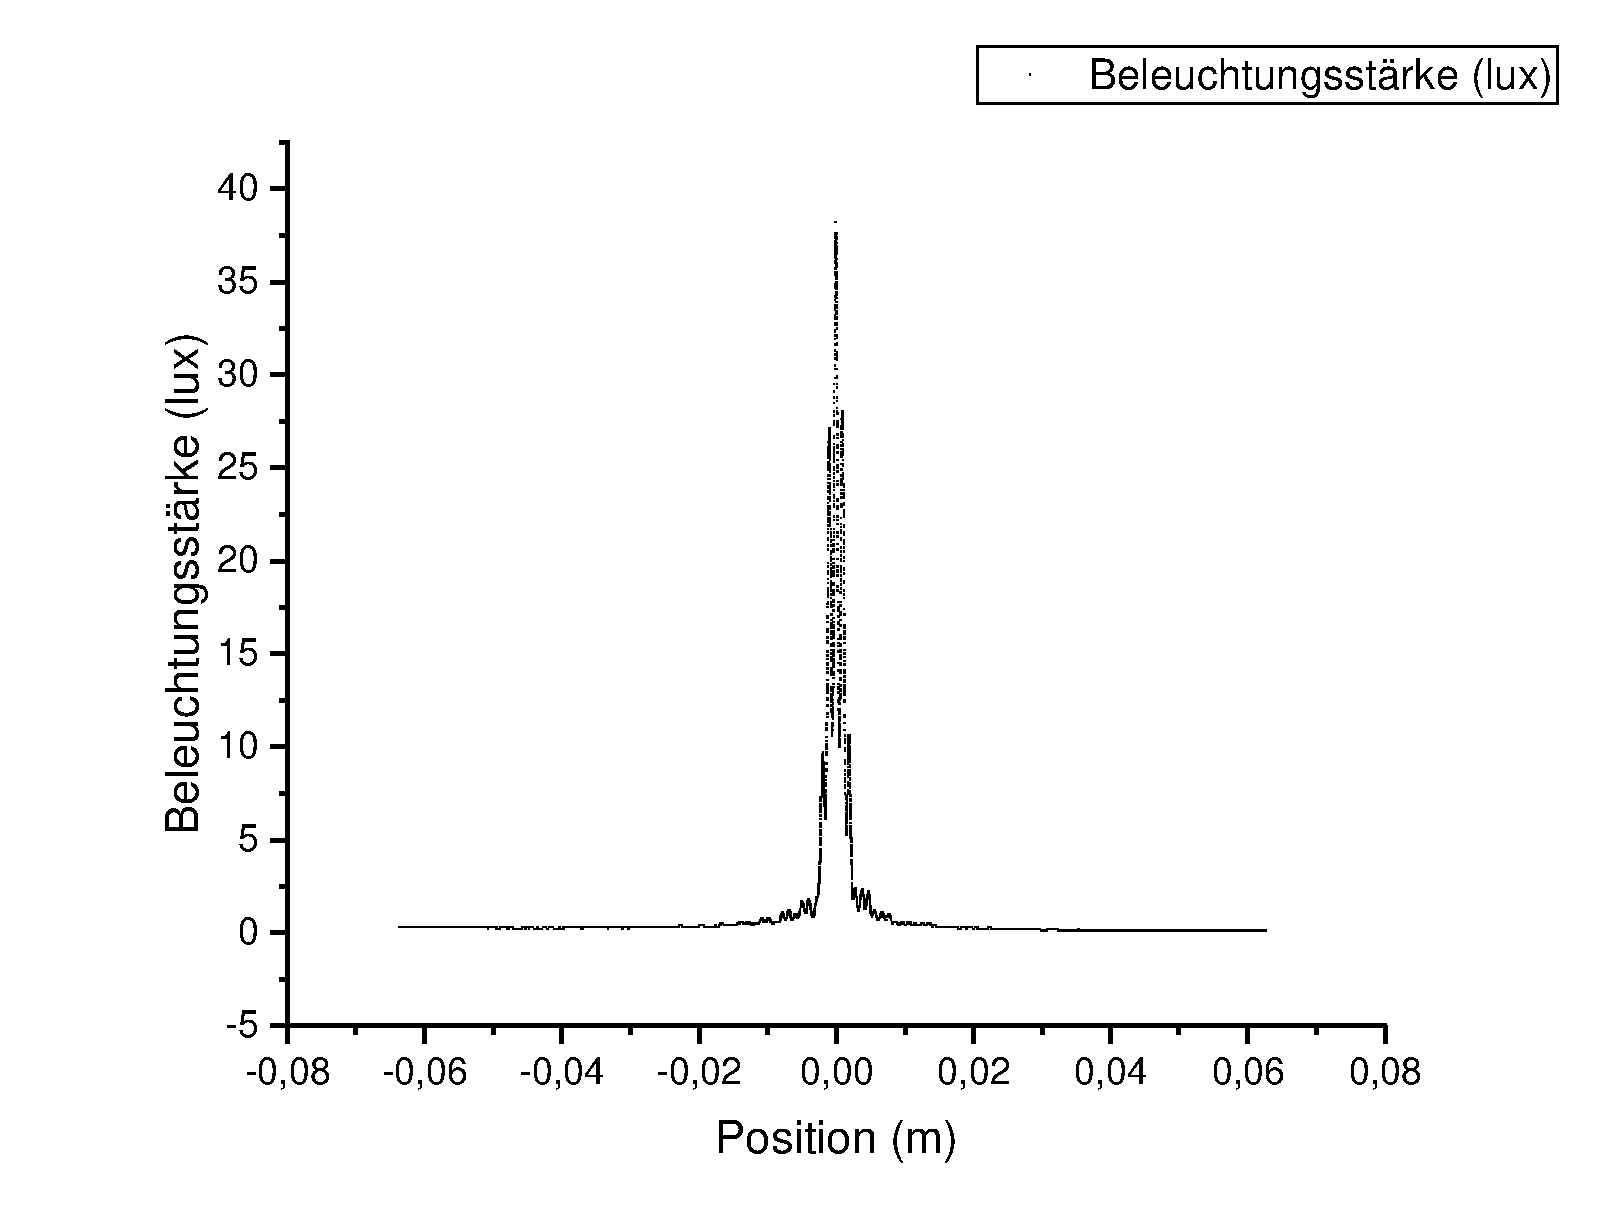
\includegraphics[width=1\linewidth]{Doppelspaltb0-15mmg0-5mmNOZOOM}
			\caption{Gesamte Messung}	
		\end{subfigure}%
		\begin{subfigure}{.5\textwidth}
			\centering
			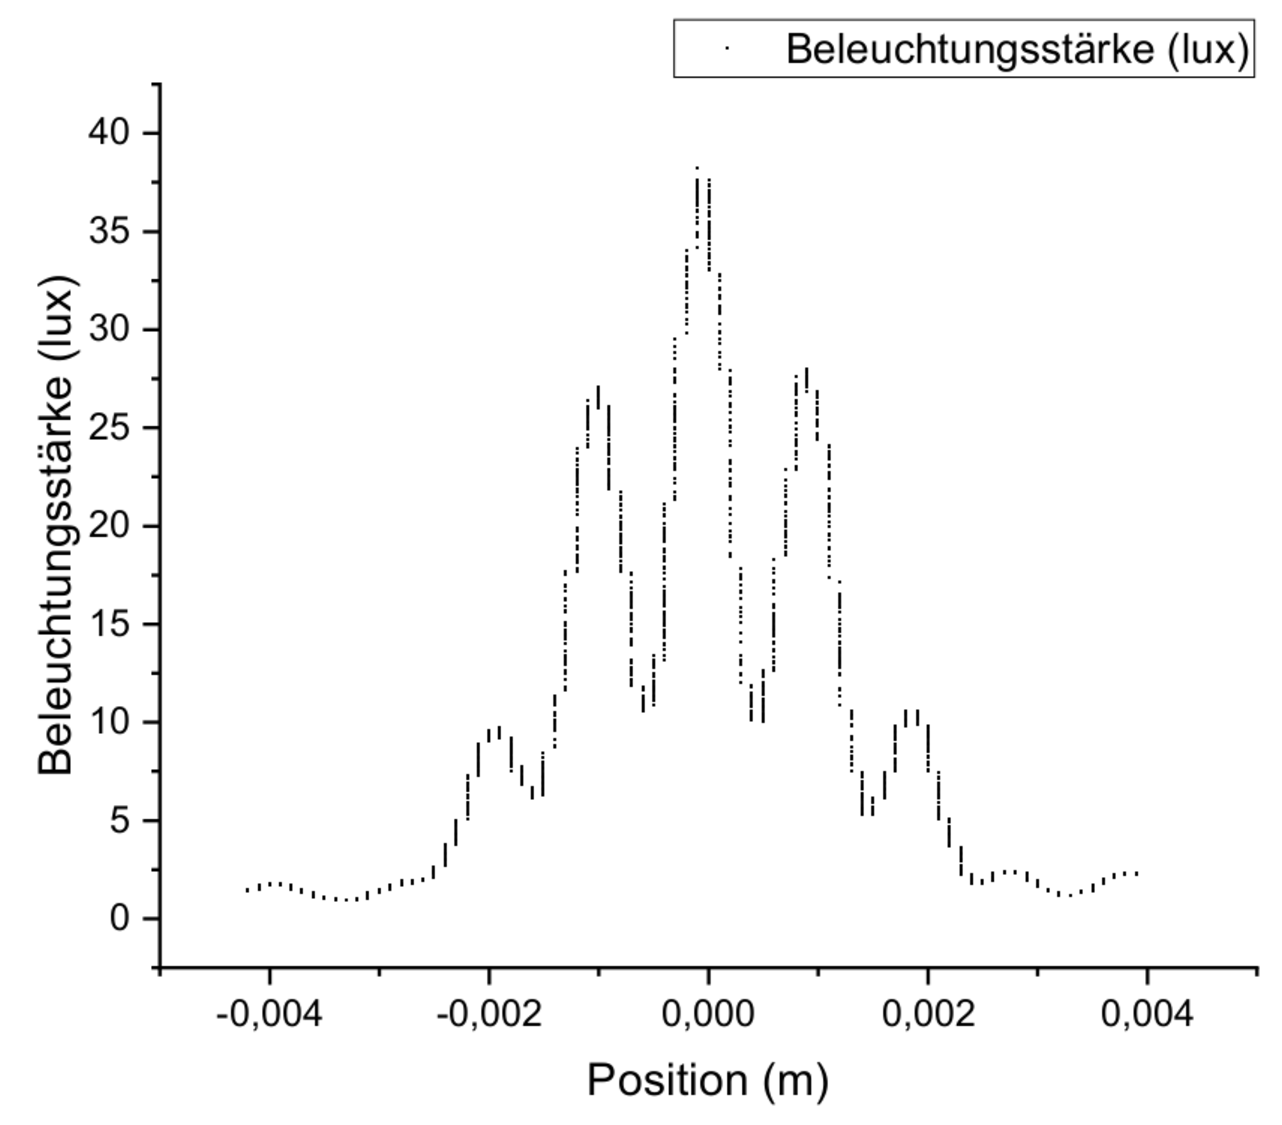
\includegraphics[width=1\linewidth]{Doppelspaltb0-15mmg0-5mm}
			\caption{Extrema niedriger Ordnung}
		\end{subfigure}
		\label{Doppelspalt0-15mm}
		\caption{Intensitätsverteilung für einen Doppelspalt mit der Spaltbreite $b = \SI{0,15}{mm}$ und $g = \SI{0,5}{mm} $ .}
	\end{figure}
	
	\subsubsection{Vergleich verschiedener Doppelspalte}
	
	\begin{figure}[H]
		\centering
		\begin{subfigure}{.5\textwidth}
			\centering
			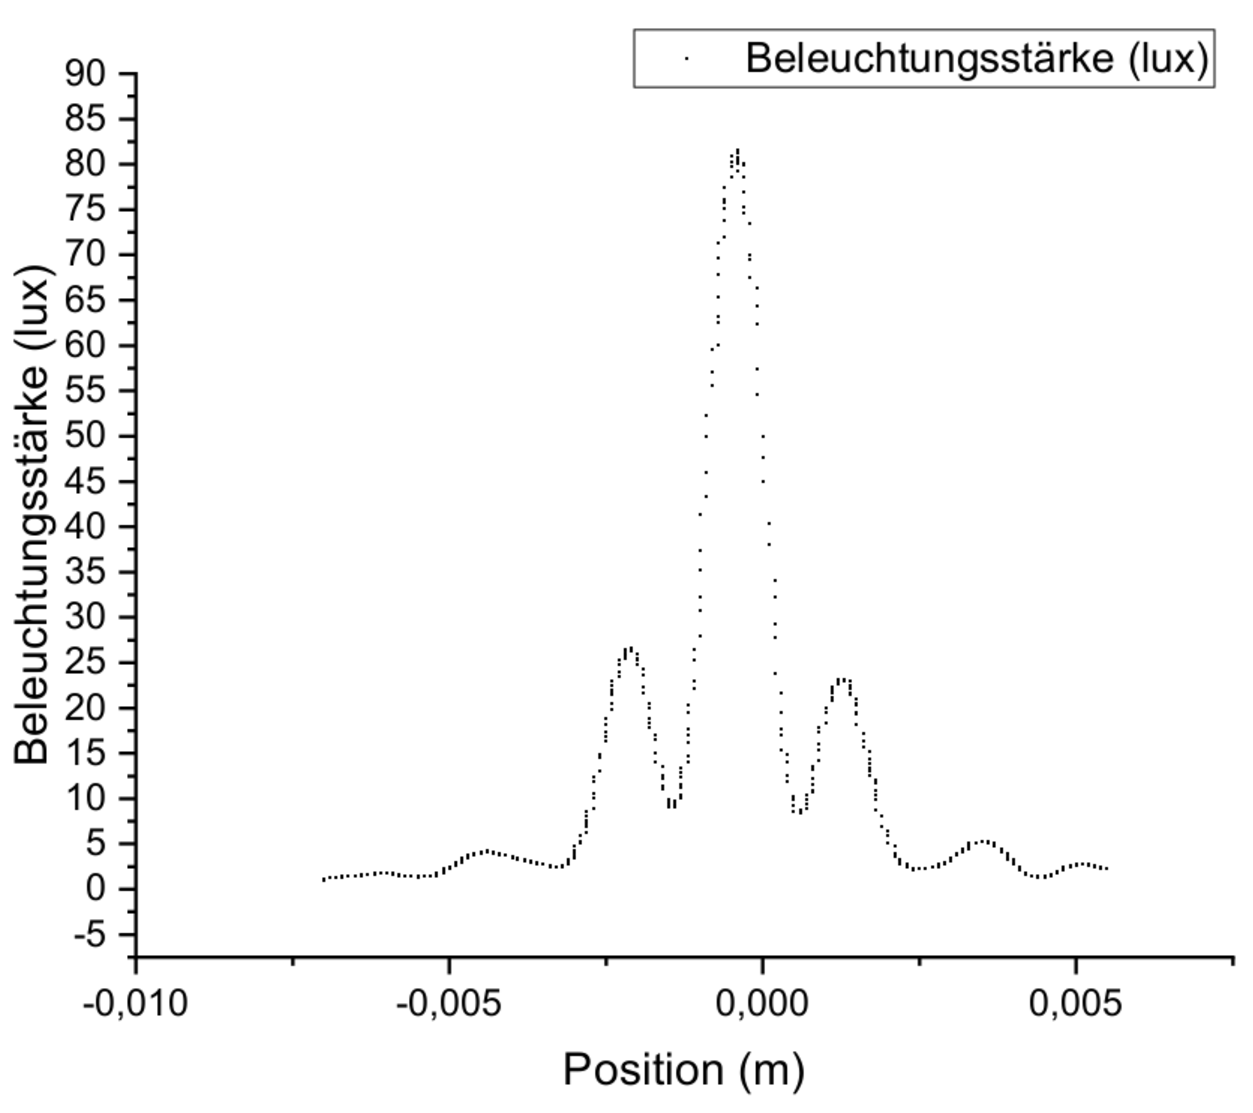
\includegraphics[width=1\linewidth]{Doppelspaltb0-15mmg0-25mm.pdf}
			\caption{$b=\SI{0,15}{mm}$, $ g=\SI{0,25}{mm}$}	
		\end{subfigure}%
		\begin{subfigure}{.5\textwidth}
			\centering
			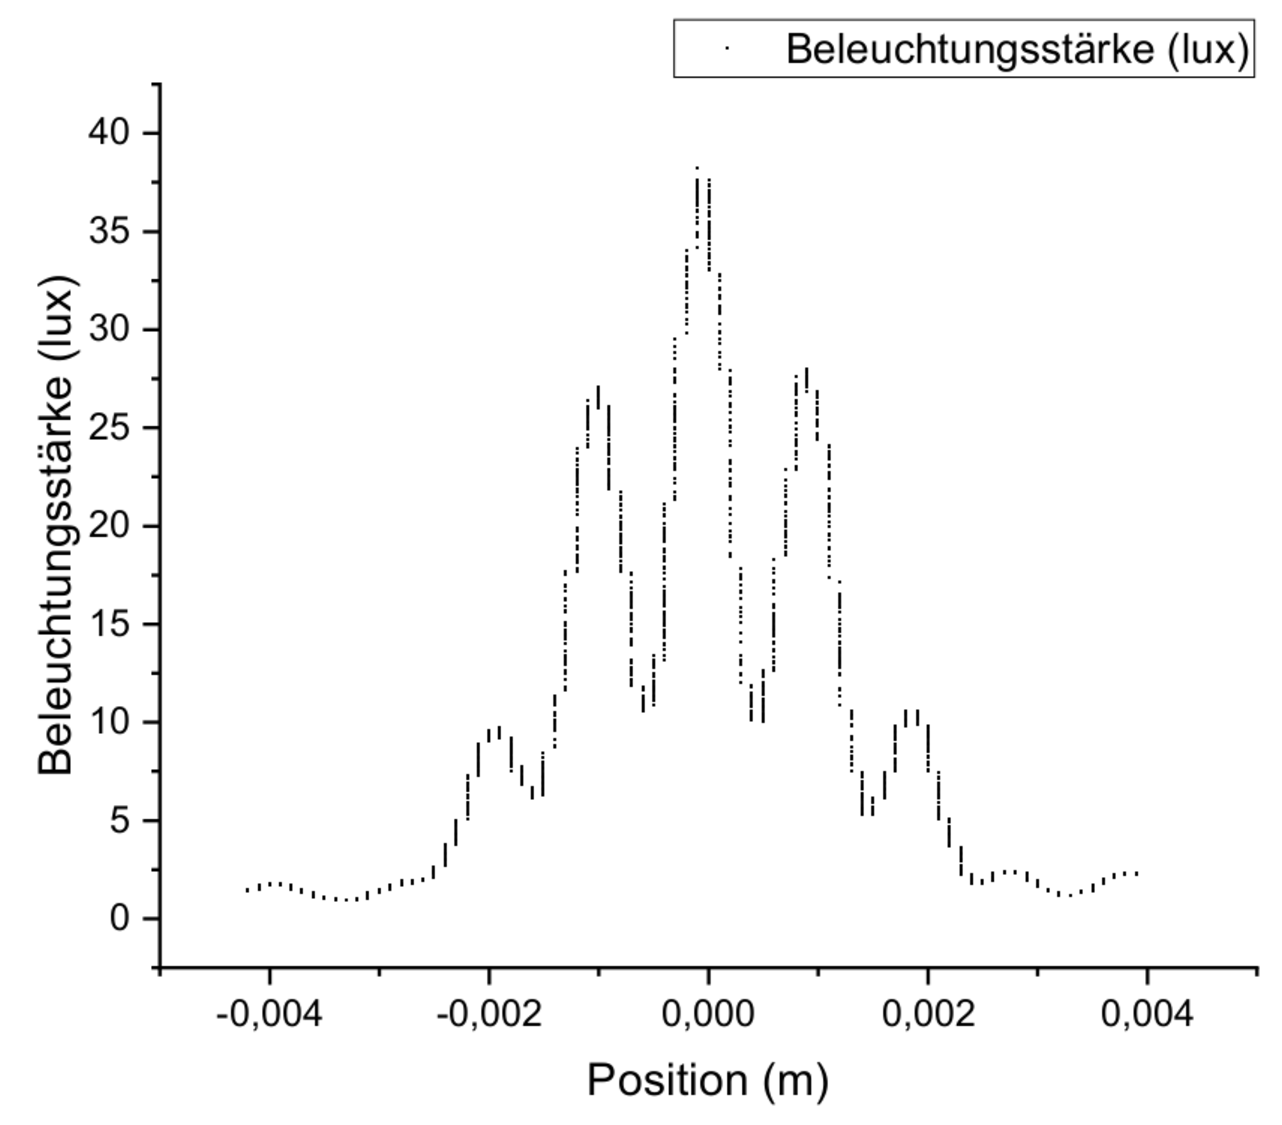
\includegraphics[width=1\linewidth]{Doppelspaltb0-15mmg0-5mm.pdf}
			\caption{$b=\SI{0,15}{mm}$, $ g=\SI{0,5}{mm}$}
		\end{subfigure}
		\begin{subfigure}{.5\textwidth}
			\centering
			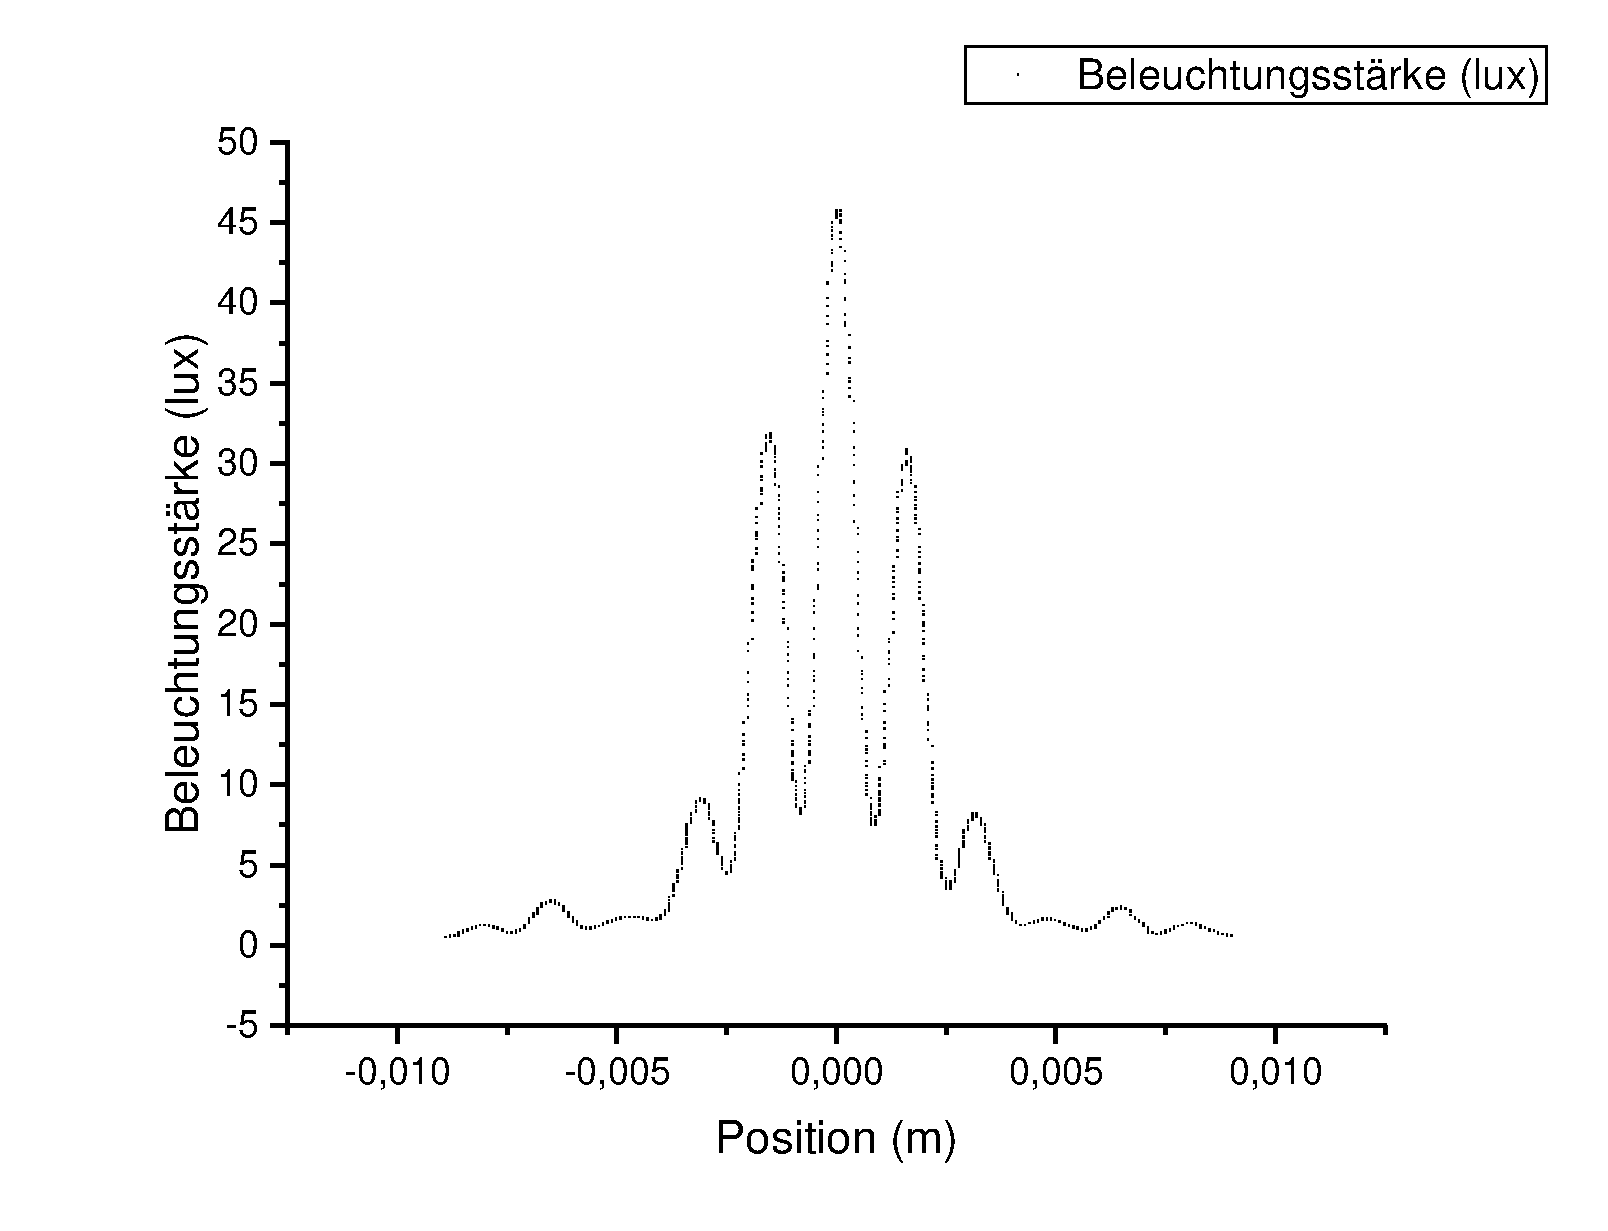
\includegraphics[width=1\linewidth]{Doppelspaltb0-10mmg0-30mm}
			\caption{$b=\SI{0,1}{mm}$, $ g=\SI{0,3}{mm}$}	
		\end{subfigure}%
		\begin{subfigure}{.5\textwidth}
			\centering
			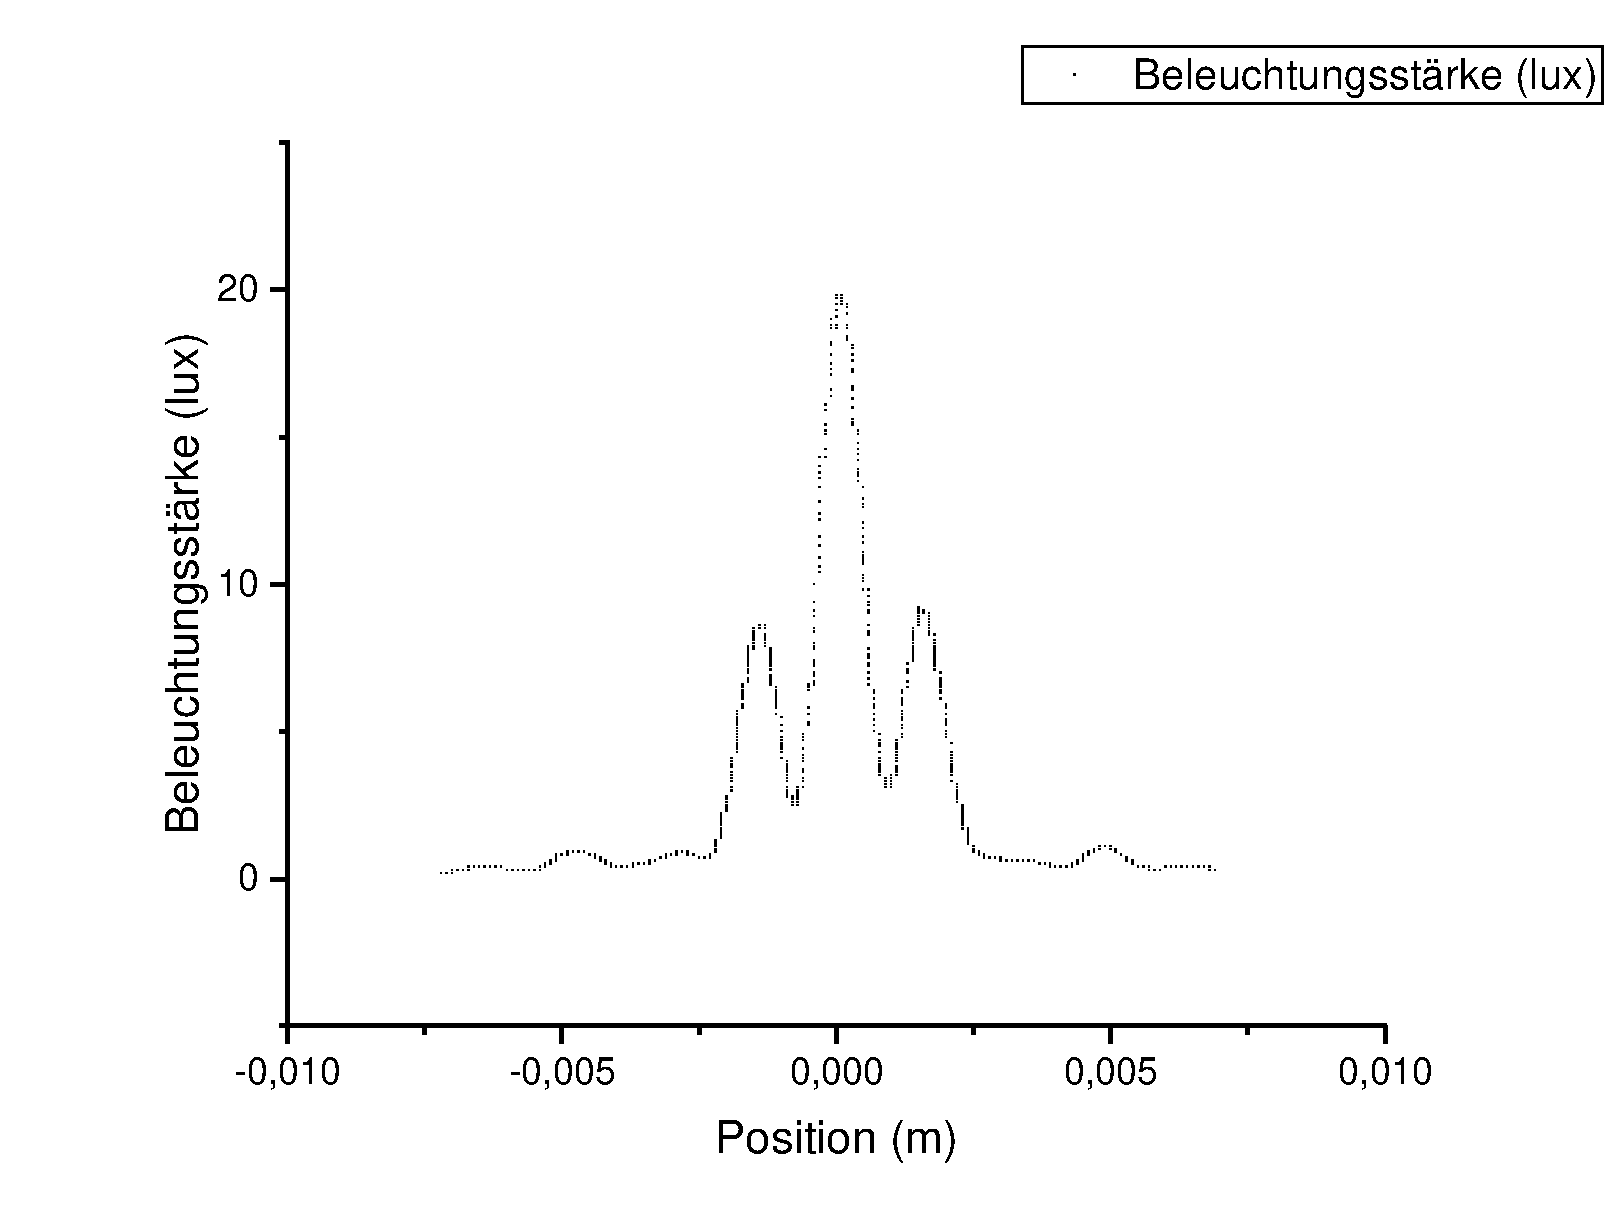
\includegraphics[width=1\linewidth]{Doppelspaltb0-15mmg0-30mm}
			\caption{$b=\SI{0,15}{mm}$, $ g=\SI{0,3}{mm}$}
		\end{subfigure}
		\caption{Intensitätsverteilungen verschiedener Doppelspalte.}
		\label{Doppelspaltvergleich}
	\end{figure}
	
	%TODO FRüh erkennbareMaxima+Minimabeim Messen
	%TODO Bezug/Nutzten oder sonst was
	%TODO auch hier die Hypothese wiederholen
	%TODO "Wo erwarten Sie die (Haupt)Maxima und Minima? "
	
	%TODO Intensitäten sind linear zu N sollten aber zu N^^2 sein
	
	\section{Schlussfolgerung}
	%TODO Rückgriff auf Hypothese und drittes Nennen dieser
	
	%TODO Quellen zitieren, Websiten mit Zugriffsdatum
	%TODO Verweise auf das Laborbuch (sind erlaubt)
	%TODO Tabelle + Bilder mit Beschriftung
	\printbibliography
\end{document}
